% 55-67(55쪽) — 이차함수 $y=f(x)$ 의 그래프와 직선 $y=x+2$(원문 「오른쪽 그림」). 스캔 화질이 낮아 TikZ 로 다시 그림.
% 라벨은 원문 것만: $x$축의 $-2$·$3$·$5$, $y$축 쪽의 $2$, $\pt{O}$, 두 그래프 이름. 점선은 원문대로 $x=3$ 에 세로로.
% 원문대로 포물선은 $x=-2$·$x=5$ 에서 $x$축과 만나고 직선과는 $x=-2$·$x=3$ 에서 만난다. 정수 $x$ 의 합(답)은 그림에서 읽히지 않는다.
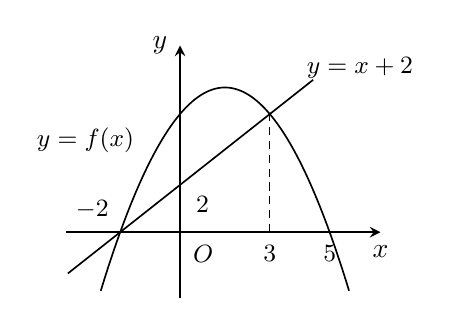
\begin{tikzpicture}[line width=0.6pt, x=0.38cm, y=0.30cm, >=stealth]
  \draw[densely dashed, line width=0.4pt] (3,0) -- (3,5);
  \draw[->, line width=0.7pt] (-3.8,0) -- (6.7,0) node[below=1pt] {$x$};
  \draw[->, line width=0.7pt] (0,-2.8) -- (0,7.9) node[left=1pt] {$y$};
  \draw[domain=-2.65:5.65, samples=90, smooth] plot (\x, {-0.5*(\x+2)*(\x-5)});
  \draw[domain=-3.75:4.45] plot (\x, {\x+2});
  \node[anchor=south east, font=\small] at (-2.05,0.15) {$-2$};
  \node[anchor=north west, font=\small] at (0.2,1.95) {$2$};
  \node[anchor=north, font=\small] at (3,-0.15) {$3$};
  \node[anchor=north, font=\small] at (5,-0.15) {$5$};
  \node[anchor=north west, font=\small] at (0.1,-0.15) {$\pt{O}$};
  \node[anchor=east, font=\small] at (-1.2,3.9) {$y=f(x)$};
  \node[anchor=south west, font=\small] at (3.9,6.1) {$y=x+2$};
\end{tikzpicture}
